\documentclass[16pt]{article}
\usepackage[english]{babel}
\usepackage{longtable}
\usepackage[top=1in, bottom=0.25in, left=1.25in, right=1.25in,includefoot,heightrounded]{geometry}
\usepackage{indentfirst}
\usepackage[utf8]{inputenc}
\usepackage{amsmath,amssymb}
\usepackage{graphicx,tikz}
\usepackage{hyperref}
\usepackage[colorinlistoftodos]{todonotes}
\usepackage[document]{ragged2e}
\usepackage{fancyhdr}
\usepackage{enumerate}
\usepackage{listings}
\usepackage{color}
\usepackage{flowchart}
\usepackage{hyperref}
\usetikzlibrary{arrows}

\usetikzlibrary{shapes.geometric, arrows}
\tikzstyle{startstop} = [rectangle, rounded corners, minimum width=3cm, minimum height=1cm,text centered, draw=black, fill=red!30]
\tikzstyle{decision} = [diamond, minimum width=4cm, minimum height=0.5cm, text centered, draw=black, fill=green!30]
\tikzstyle{process} = [rectangle, minimum width=3cm, minimum height=1cm, text centered, draw=black, fill=orange!30]
\tikzstyle{arrow} = [thick,->,>=stealth]
\tikzstyle{io} = [trapezium, trapezium left angle=70, trapezium right angle=110, minimum width=2cm, text width=4cm, minimum height=1cm, text centered, draw=black, fill=blue!30]

\pagestyle{fancy}
\fancyhf{}
\lhead{Myles Deslippe}
\rhead{Comp 3300 | Operating System Fundamentals}
\cfoot{\thepage}

\definecolor{MyDarkGreen}{rgb}{0.0,0.4,0.0}
\lstset{inputencoding=ansinew}
\lstset{breaklines=true} 

\begin{document}

    \section*{\centering{System Structure}}

    \subsection*{The User Interface}
    \begin{itemize}
        \item \textbf{Operating systems} provide an \textbf{environment} for the \textbf{execution of programs}, and \textbf{services to those programs}.
        \item One set of \textbf{operating system services provides functions} that are helpful to the \textbf{user}.
        \item The \textbf{user interface} is the way \textbf{users interact with the operating system}.
        \item There are \textbf{two types} of \textbf{user interfaces}:
        \begin{enumerate}
            \item The \textbf{command-line interface (CLI)} is a way the \textbf{user} can \textbf{interact} with the \textbf{operating system} through a set of \textbf{commands}.
            \item The \textbf{graphical user interface (GUI)} is a way the \textbf{user} can \textbf{interact} with the \textbf{operating system} in a \textbf{graphical environment}.
        \end{enumerate}
        \item Any operating system \textbf{user interface} should allow the user to \textbf{perform file-system manipulation}, \textbf{execute programs}, and \textbf{interact with IO devices}.
        \item Additionally, the \textbf{user interface} should handle \textbf{error detection, resource allocation, and device security} behind the scenes.
        \item[] 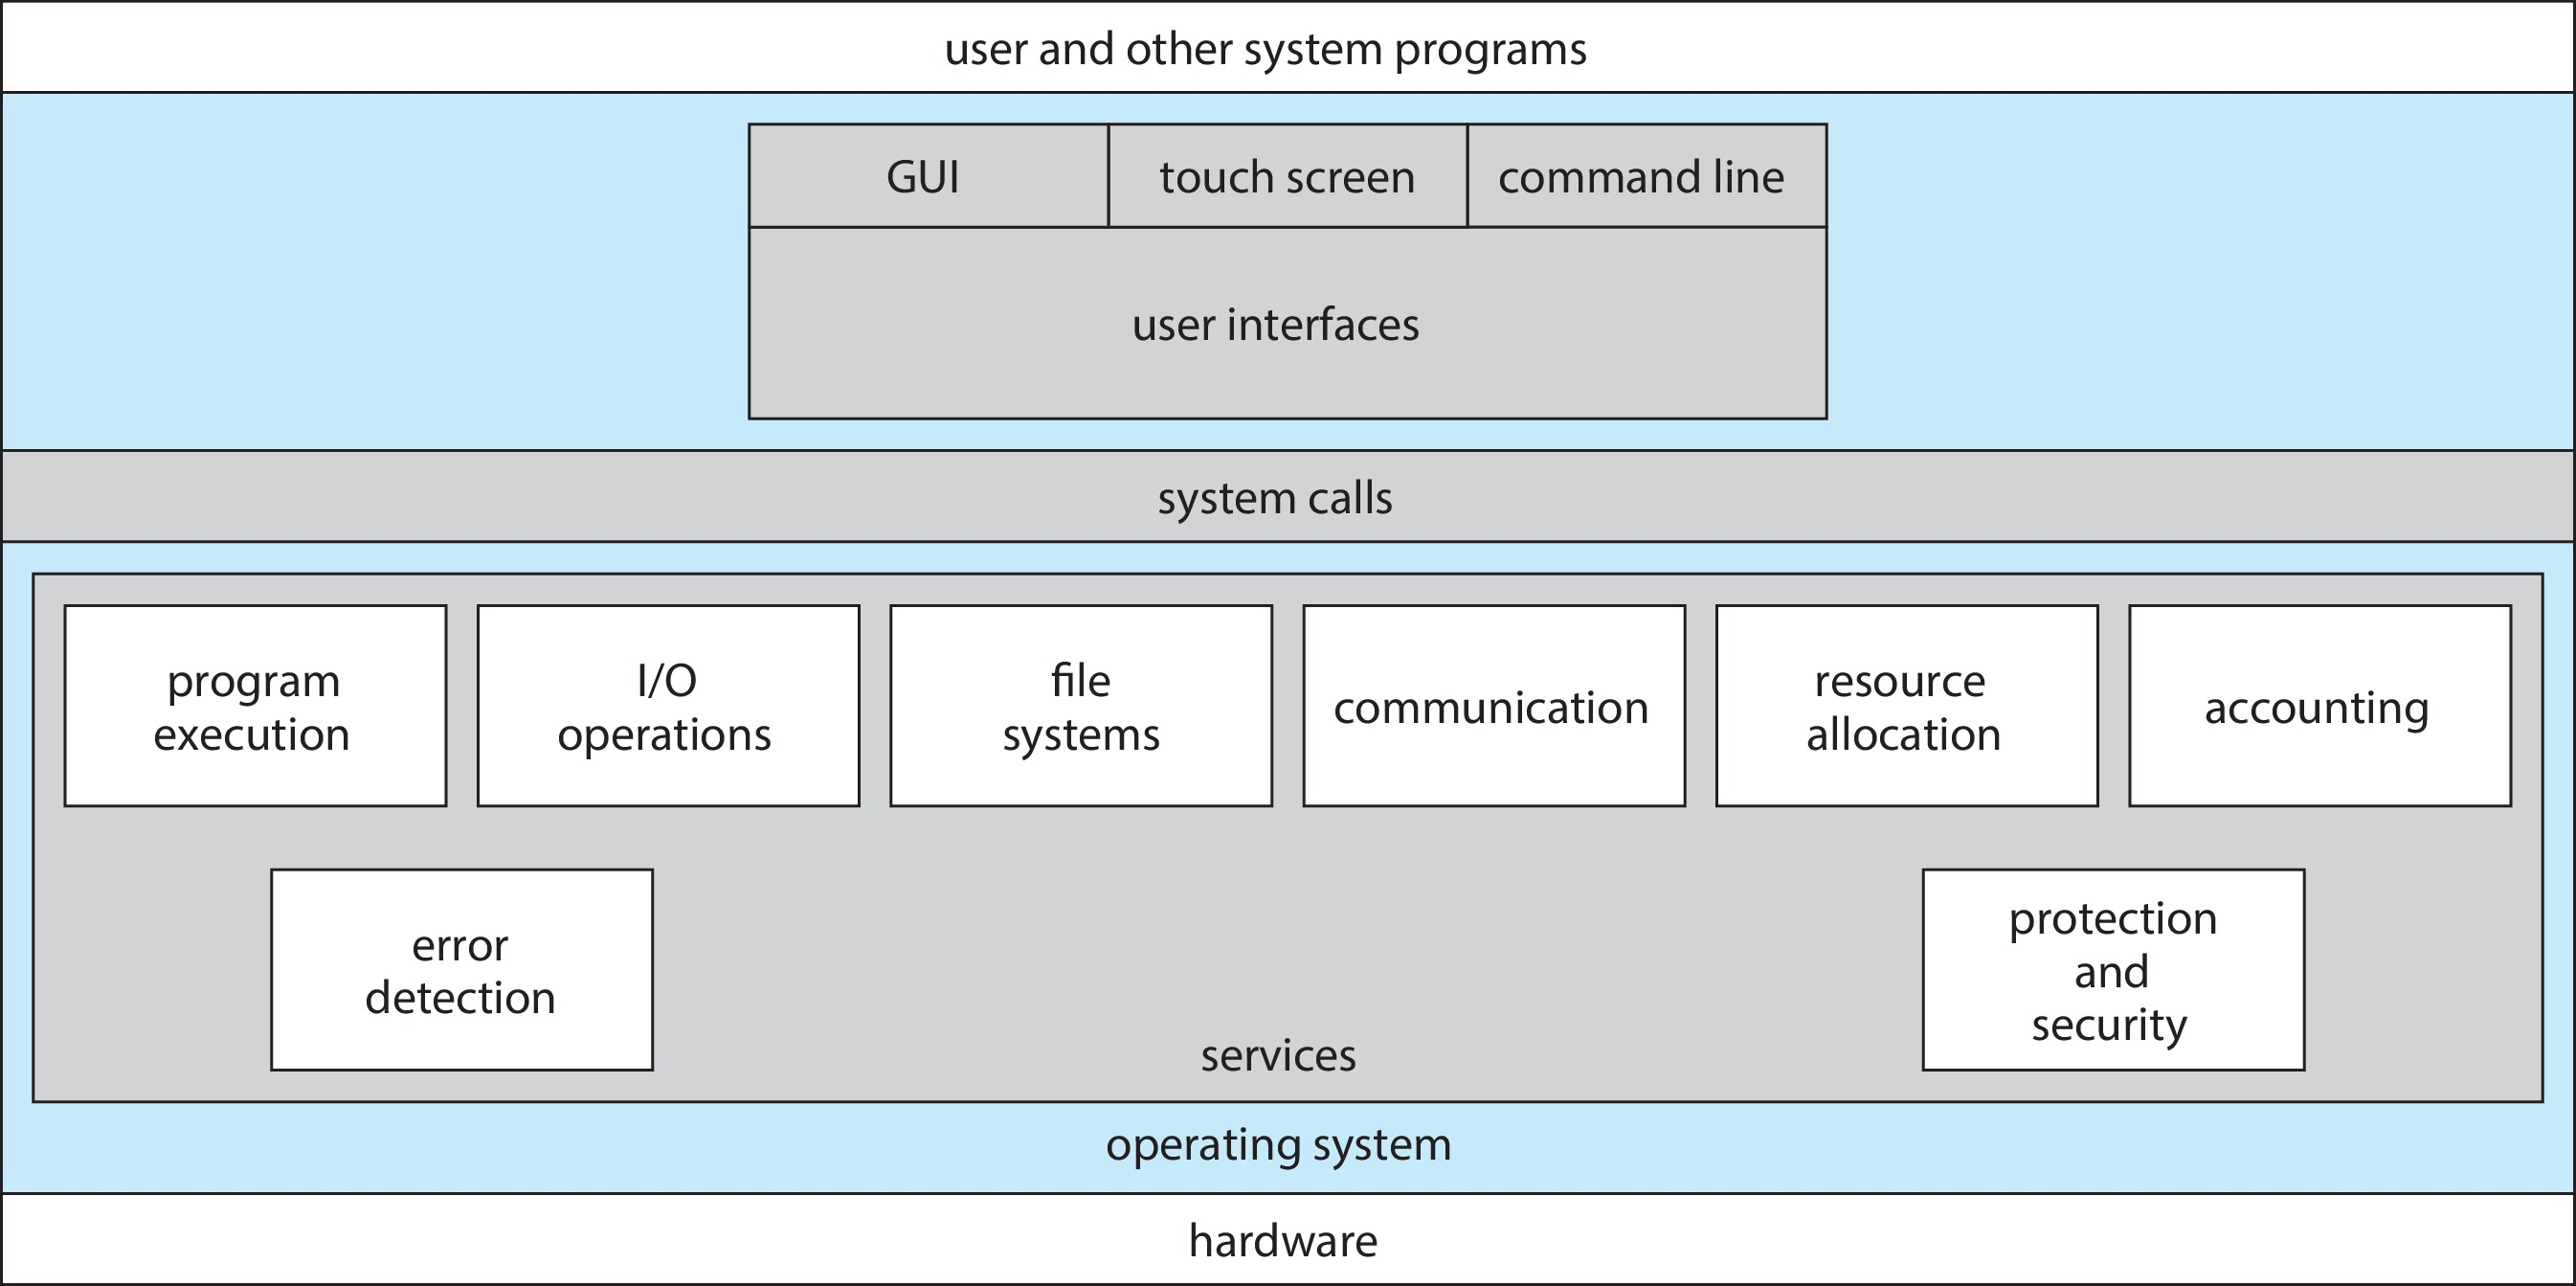
\includegraphics[height=200px]{images/User-Interface.jpg}
    \end{itemize}

    \subsection*{System Calls}
    \begin{itemize}
        \item A \textbf{system call} is a \textbf{programming interface} to the \textbf{services} provided by the \textbf{operating system}.
        \item \textbf{System calls} are invoked with the system's \textbf{assembly language}.
        \item To make \textbf{software development easier} operating systems typically provide a \textbf{high-level programming interface} that \textbf{abstracts} the \textbf{system calls}.
        \begin{itemize}
            \item \textbf{Windows systems} use the \textbf{Win32 API}.
            \item \textbf{POSIX-based systems} (UNIX, Linux, MacOS, etc) use the \textbf{POSIX API}.
        \end{itemize}
        \item \textbf{System calls} typically require \textbf{parameters}. There are \textbf{three methods} that can be used to \textbf{pass parameter to the operating system}:
        \begin{enumerate}
            \item Pass the parameters in registers. (Max amount of parameters is restricted to register count)
            \item Store the parameters in a block / table that is in the system's primary memory, and pass the memory location of the table in a register. (Used by Linux)
            \item Push the parameters onto the stack, and the operating system will pop them off.
        \end{enumerate}
        \begin{itemize}
            \item Method 2 and 3 \textbf{do not have a maximum amount of parameters}.
        \end{itemize}
        \item \textbf{System calls} are needed for: \textbf{process control, file management, device management, information maintenance, communication, and permission management}.
    \end{itemize}

    \subsection*{System Programs}
    \begin{itemize}
        \item \textbf{System programs} can be thought of a \textbf{bundles} of \textbf{system calls} that provide basic functionality to \textbf{users} so they do not need to write their own programs to solve common problems.
        \item A \textbf{daemon} is a \textbf{system program} that runs as a \textbf{background process}, and usually provides some type of service.
    \end{itemize}

    \subsection*{Separation of Mechanism and Policy}
    \begin{itemize}
        \item An operating system \textbf{policy} is a way of choosing an \textbf{action to perform}.
        \item An operating system \textbf{mechanism} is the \textbf{implementation} that \textbf{enforces a policy}.
        \item \textbf{Policies and mechanism should be separated}. The policy remains the same, but the \textbf{mechanism may vary} depended on the type of system the operating system is running on.
    \end{itemize}

    \subsection*{Monolithic and Modular Operating Systems}
    \begin{itemize}
        \item A \textbf{monolithic operating system} (tightly-coupled system) is an operating system that uses \textbf{one static-compiled image} and runs in an \textbf{all or nothing mode}.
        \item A \textbf{layered operating system} is an operating system that is divided into several layers with each layer interfacing with the one below it. The first layer (Layer 0) is the hardware, and the final layer (Layer N) is the user interface.
        \item The \textbf{layered approach} has a lot of \textbf{overhead} because each user functionality has to \textbf{traverse all of the layers}.
        \item A \textbf{modular operating system} (loosely-coupled system) is an operating system that is built with various tasks \textbf{divided} into \textbf{distinct processes} each of which contain their own \textbf{interface}.
        \begin{itemize}
            \item One way to implement a \textbf{modular operating system} is with a \textbf{microkernel}. This approach contains a kernel that is the \textbf{near-minimum amount of software that can provide methods to implement an operating system}. \textbf{Modules} are built on top of \textbf{microkernel}, and communicate with each-other with \textbf{message passing} through the kernel.
            \item \textbf{Microkernels} are generally more \textbf{secure, reliable, and maintainable}. The only downside is that \textbf{modular communication has more overhead}.
        \end{itemize}
        \item \textbf{Modular operating systems} use \textbf{Loadable Kernel Modules (LKM)} which gives the operating system the ability to \textbf{add or remove modules at runtime} without the need to recompile the kernel or restart the system.
        \item \textbf{Monolithic operating systems} are \textbf{difficult to implement and maintain}, but have \textbf{less overhead}.
        \item You can also have a \textbf{hybrid operating system} which is partially \textbf{monolithic} and \textbf{modular}.
    \end{itemize}

\end{document}